% This is the October Version without appendices. The October Version
% remains the authoritative text. We've taken out some math for BJPS,
% not just the appendices. Differentiation of DKL. Definition of the
% powerset approach.

% This is what I call the ``October Version'' which is an attempt to
% reduce both word count and technical nature of the piece significantly
% in order to be more publishable. For the more technical and wordier
% version see the ``Episteme Version.'' 

% This is an edited version of
% 2011__Stefan_Lukits__The_Principle_of_Maximum_Entropy_and_a_Problem_in_Probability_Kinematics.tex
% Some interesting material from the 2011 file is missing, because we
% had to reduce the word count. On the other hand, the information is
% condensed, improved, and there is some additional material on
% Halpern and Gruenwald's CAR. I would run a diff and scan the
% relevant sections of the 2011 file to see the missing paragraphs,
% but use this one for further projects.

\documentclass[12pt]{article}
\usepackage{october}

\begin{document}

% \title{The Principle of Maximum Entropy and a Problem in Probability Kinematics}

% \author{Stefan Lukits}
% \date{}

% \maketitle

% \doublespacing

\newcounter{chap}

\setcounter{chap}{1}

{\noindent} \textsc{The Principle of Maximum Entropy \newline and a Problem in
Probability Kinematics}

\begin{abstract}
  \noindent Given a more general type of evidence than required for
  Bayes' formula, the principle of maximum entropy (\textsc{maxent})
  provides a unique solution for the posterior probability
  distribution based on the intuition that the information gain
  consistent with assumptions and evidence should be minimal.
  Opponents of objective methods to determine these probabilities
  prominently cite van Fraassen's Judy Benjamin case to undermine the
  generality of the \textsc{maxent}. The article shows that an
  intuitive approach to Judy Benjamin's case that on account of
  independence assumptions should support the opponents turns out to
  support \textsc{maxent}. It also demonstrates that opponents
  improperly apply independence assumptions to the problem.
\end{abstract}

% \begin{abstract}
%   \noindent Given a set of probabilities on an event space and a new
%   observation, it is common to form updated probabilities by using
%   rules of conditioning. Some observations pose constraints that
%   cannot be addressed by standard conditional probabilities or Jeffrey
%   conditioning. The principle of maximum entropy (abbreviated
%   \textsc{maxent}) claims that it is then appropriate to form an
%   updated probability assessment by minimizing information gain
%   consistent with the observation. Opposition to the \textsc{maxent}
%   leans heavily on one counterexample: the Judy Benjamin problem. This
%   article shows that an intuitively plausible approach that should
%   support the opponents' case turns out to support the
%   \textsc{maxent}. It becomes apparent that the opponents improperly
%   apply independence assumptions to the problem.
% \end{abstract}

% \begin{abstract}
%   When we have a set of prior probabilities and make an observation,
%   we use probability updating or conditioning to provide a set of
%   posterior probabilities. If we attain the new information in the
%   form of an event, the use of conditional probabilities is a widely
%   accepted form of arriving at appropriate posterior probabilities.
%   Sometimes the information does not come in the form of an event and
%   Jeffrey conditioning can be used. Some observations pose affine
%   constraints that cannot even be addressed by Jeffrey conditioning.
%   The Principle of Maximum Entropy (PME) claims that in this case it
%   is appropriate to form a posterior probability assessment by
%   minimizing the information gain with respect to the prior
%   probabilities that is consistent with the evidence. There is strong
%   opposition to the PME, some of which leans heavily on one particular
%   counterexample: the Judy Benjamin problem. This article shows that a
%   new approach that, based on its independence assumptions, should
%   support the opponents' case turns out to support the PME. In
%   addition, the article demonstrates by providing counterexamples that
%   independence assumptions commonly made by opponents are improperly
%   applied to the problem.
% \end{abstract}

% word count (* 456 13.7) 6247
% abstract: 104
% main text: 4378
% references: 489
% appendix: 332

% \newpage

% \noindent \textsc{The Principle of Maximum Entropy \newline and a Problem in Probability Kinematics}

% \bigskip

\kapt{Introduction}

\smallskip

% \begin{quotex}
%   Acknowledgments: Thanks to James Baugh at the Mathematics Department
%   at GCSU in Milledgeville, GA, for helping me when I was stuck with
%   an integral. Somebody hiding behind the pseudonym micromass helped
%   me with a binomial identity on physicsforums.com. Thanks to
%   Jan-Willem Romeijn, Adom Giffin, and Paul Bartha for comments in
%   writing and the many verbal comments from participants at the 2011
%   meeting of the Canadian Society for the History and Philosophy of
%   Science in Fredericton, NS. Thank you to my students at Vancouver
%   Community College. Thank you to Donat Berghuber, who taught me 0.95
%   of the mathematical skills I needed for this paper.
% \end{quotex}

\nias Probability kinematics is the field of inquiry asking how we
should update a given probability distribution in the light of
evidence. If the evidence comes in the form of an event, it is
relatively uncontroversial to use conditional probabilities (call this
standard conditioning). Sometimes, however, the evidence may not
relate the certainty of an event but a reassessment of its uncertainty
or its probabilistic relation to other events (see
\scite{8}{jeffrey65}{153ff}), expressible in a shift in expectation
(see \scite{7}{hobson71}{}). Bas van Fraassen has come up with an
example from the 1980 comedy film \emph{Private Benjamin} (see van
Fraassen 1981)\nonsc{}, in which Goldie Hawn portrays a
Jewish-American woman (Judy Benjamin) who joins the U.S. Army.

\begin{figure}[h]
  \begin{flushright}
    \begin{minipage}[h]{.8\linewidth}
      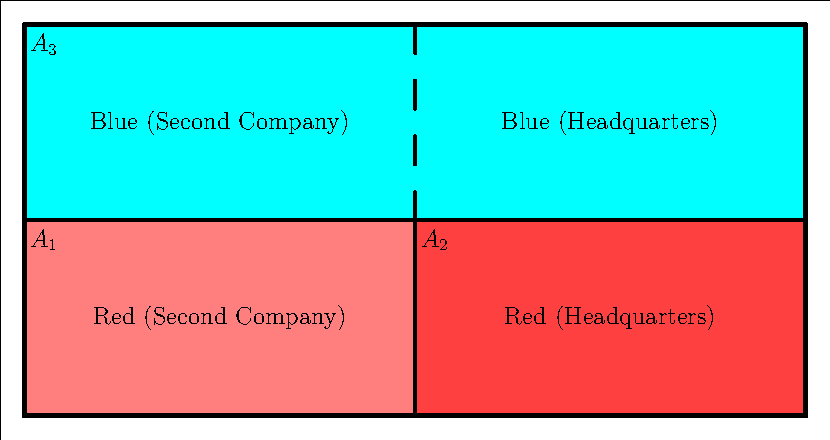
\includegraphics[width=\textwidth]{judy.pdf}
      \caption{Judy Benjamin's map. Blue territory ($A_{3}$) is friendly and
        does not need to be divided into a Headquarters and a Second
        Company area.}
      \label{fig:map}
    \end{minipage}
  \end{flushright}
\end{figure}

In van Fraassen's interpretation of the movie, Judy Benjamin is on an
assignment and lands in a place where she is not sure of her location.
She is on team Blue. Because of the map, her probability of being in
Blue territory equals the probability of being in Red territory, and
being in the Red Second Company area equals the probability of being
in the Red Headquarters area. Her commanders inform Judy by radio that
in case she is in Red territory, her chance of being in the Red
Headquarters area is three times the chance of being in the Red Second
Company area.

At the heart of our investigation are two incompatible but
independently plausible intuitions regarding Judy's choice of updated
probabilities for her location (much more in the next section). First
we note, however, that there is no immediately obvious event space in
which we can condition on an event of which we are certain. Grove and
Halpern \scite{1}{grovehalpern97}{} have written an article on how to
construct such event spaces and then condition on the event that Judy
Benjamin receives the information that she receives from her
commanders. They admit, however, that the construction of such spaces
(sometimes called retrospective conditioning) is an exercise in
filling in missing details and supplying information not contained in
the original problem.

If we assume that the attempt fails to define an event on which Judy
Benjamin could condition her probabilities, we are left with two
possibilities. Her new information (it is three times as likely to
land in $A_{2}$ than to land in $A_{1}$, see figure~\ref{fig:map} and
the details of the problem in the next section) may mean that we have
a redistribution of a complete partition of the probabilities. This is
called Jeffrey conditioning and calls for Jeffrey's rule. Jeffrey's
rule is contested in some circles, but we will for this project accept
its validity in probability kinematics. We will see in what follows
that some make the case that Jeffrey conditioning is the correct way
to solve the Judy Benjamin problem.

The third possibility to solve this problem (after standard
conditioning and Jeffrey's rule) is to consult a highly contested
procedure to find an objective updating procedure in case the first
two scenarios do not apply: the principle of maximum entropy (from now
on \textsc{maxent} for abbreviation). \textsc{maxent} can be applied
to any situation in which we have a completely quantified probability
distribution and an affine constraint (we will explain the nature of
affine constraints in more detail later). If our new evidence is the
observation of an event (or simply certainty about an event that we
did not have previously), then the event provides an affine constraint
and can be used for updating by means of standard conditioning. If our
new evidence is a redistribution of probabilities where we can apply
Jeffrey's rule, then the redistribution provides an affine constraint
and can be used for updating by means of Jeffrey's rule. These two
possibilities, however, do not exhaust affine constraints. The Judy
Benjamin problem illustrates the third possibility where the affine
constraint only redistributes some groups of probabilities and leaves
open the question how this will affect the probabilities not included
in this redistribution.

Advocates of \textsc{maxent} claim that in this case the probabilities
should be adjusted so that they are minimally affected (we make this
precise by using information theory) while at the same time according
with the constraint. Opponents of this view grant that \textsc{maxent}
is an important tool of probability kinematics, but that results of
\textsc{maxent} that are difficult to accept (such as the Judy
Benjamin problem) urge us to embrace a more pluralistic,
situation-specific methodology.

Joseph Halpern, for example, writes in \emph{Reasoning About
  Uncertainty} that \qeins{there is no escaping the need to understand
  the details of the application} \scite{2}{halpern03}{423} and
concludes that \textsc{maxent} is a valuable tool, but should be used
with care (see \scite{8}{grovehalpern97}{110}), explicitly basing his
remark on the counterintuitive behaviour of the Judy Benjamin problem.
Diaconis and Zabell state \qeins{that any claims to the effect that
  maximum-entropy revision is the only correct route to probability
  revision should be viewed with considerable caution}
\scite{2}{diaconiszabell82}{829}. \qeins{Great caution} (1994, 456) is
also what Colin Howson and Allan Franklin advise about the more basic
claim that the updated probabilities provided by \textsc{maxent} are
as like the original probabilities as it is possible to be given the
constraints imposed by the data.

Igor Douven and Jan-Willem Romeijn agree with Richard Bradley that
\qeins{even Bayes' rule \qzwei{should not be thought of as a universal
    and mechanical rule of updating, but as a technique to be applied
    in the right circumstances, as a tool in what Jeffrey terms
    \emph{the art of judgment}.} In the same way, determining and
  adapting the weights [epistemic entrenchment] supposes, or deciding
  when Adams conditioning applies, may be an art, or a skill, rather
  than a matter of calculation or derivation from more fundamental
  epistemic principles} \scite{2}{douvenromeijn09}{16} (for the
Bradley quote see \scite{8}{bradley05}{362}).

% Teddy Seidenfeld gives his own reasons why he is not an objective
% Bayesian in an article entitled \qeins{Why I Am Not an Objective
%   Bayesian} \scite{1}{seidenfeld79}{} (claiming that in particular
% circumstances involving noise factors \textsc{maxent} will
% inappropriately provide more information based on less evidence). Jos
% Uffink targets especially Shore and Johnson's assumptions when they
% identify \textsc{maxent} as the unique method of determining updated
% probability distributions, given certain types of constraints. Uffink
% shows how a more reasonable restatement of Shore and Johnson's
% assumptions results in a whole class of updating procedures, the
% so-called R{\'e}nyi entropies (see \scite{7}{uffink95}{}). This also
% appears to be van Fraassen's conclusion when he suggests that
% \textsc{maxent} is a special instance of a family of principles which
% are consistent relative to specified assumptions (see van Fraassen et
% al.\ 1986)\nonsc{}. Dias and Shimony provide a very interesting case of
% failure for \textsc{maxent} that we will not address in this paper
% because it is not relevant to the Judy Benjamin problem (see
% \scite{7}{diasshimony81}{}), although we hope to address it at a later
% date.

What is lacking in the literature is an explanation by \textsc{maxent}
advocates of the counterintuitive behaviour of the cases repeatedly
quoted by their adversaries. This is especially surprising as we are
not dealing with an array of counter-examples but only a handful, the
Judy Benjamin problem being prime among them. In Halpern's textbook,
for example, the reasoning is as follows: \textsc{maxent} is a
promising candidate which delivers unique updated probability
distributions; but, unfortunately, there is counterintuitive behaviour
in one specific case, the Judy Benjamin case (see
\scite{8}{halpern03}{110, 119}); therefore, we must abide by the
eclectic principle of considering not only \textsc{maxent}, but also
lower and upper probabilities, Dempster-Shafer belief functions,
possibility measures, ranking functions, relative likelihoods, and so
forth. The human inquirer is the final arbiter between these
conditionalization methods.

We will undermine the notion that \textsc{maxent}'s solution for the
Judy Benjamin problem is counterintuitive. The intuition that
\textsc{maxent}'s solution for the Judy Benjamin problem violates
(call it T1) is based on fallacious independence and uniformity
assumptions. There is another powerful intuition (call it T2) in
direct contradiction to T1 which \textsc{maxent} obeys. Therefore,
Halpern does not give us sufficient grounds for the eclecticism
advocated throughout his book. We will show that another intuitive
approach, the powerset approach, lends significant support to the
solution provided by \textsc{maxent} for the Judy Benjamin problem,
especially in comparison to intuition T1, many of whose independence
and uniformity assumptions it shares.

Dealing in stereotypes for a moment, there is a long-standing
disagreement between philosophers on the one hand and physicists on
the other hand whether (the philosophers) updating probabilities is
irreducibly accompanied by thoughtful deliberation choosing between
approaches depending on individual problems, or (the physicists)
problems are ill-posed if they do not contain the information
necessary to let a non-arbitrary, objective process arrive at a
unique updated probability distribution. In the literature, Judy
Benjamin serves as an example to defend in favour of the philosophers
what I shall call the full employment theorem of probability
kinematics.

The full employment theorem of probability kinematics claims that
\textsc{maxent} is only one of many different strategies to update
probabilities. In order to decide which strategy is the most
appropriate for your problem you need a resident formal epistemologist
to do the thinking and weigh the intuitions for you. For a fee, of
course. Thus formal epistemologists will always be fully employed.
(E.T. Jaynes makes similar observations when he derisively talks about
the statistician-client relationship as one between a doctor and his
patient, see \scite{8}{jaynes98}{492 and 506}.) There is an analogous
full employment theory in computer science about writing computer
programs which has been formally proved to be true. Our contention is
that no such proof is forthcoming in probability kinematics. The case
rests in a significant measure (see Halpern's book) on a
counterexample to \textsc{maxent}, the Judy Benjamin problem. We show
in this article that our intuitions are initially misguided about the
Judy Benjamin problem because we make independence and uniformity
assumptions that on closer examination are not tenable.

\medskip

\kapt{Two Intuitions}

\smallskip

\nias There are two pieces of information relevant to Judy Benjamin
when she decides on her updated probability assignment. We will call
them ({\ref{eq:map}}) and ({\ref{eq:hdq}}). As in
figure~\ref{fig:map}, $A_{1}$ is the Red Second Company area, $A_{2}$ is
the Red Headquarters area, $A_{3}$ is Blue territory. Judy presumably
wants to be in Blue territory, but if she is in Red territory, she
would prefer their Second Company area (where enemy soldiers are not
as well-trained as in the Headquarters area).

\begin{enumerate}
\item[({\ref{eq:map}})] Judy has no idea where she is. She is on team Blue.
  Because of the map, her probability of being in Blue territory
  equals the probability of being in Red territory, and being in the Red
  Second Company area equals the probability of being in the Red
  Headquarters area.
\item[({\ref{eq:hdq}})] Her commanders inform Judy that in case she is in Red
  territory, her chance of being in their Headquarters area is three
  times the chance of being in their Second Company area.
\end{enumerate}

\nial In formal terms (sloppily writing $A_{i}$ for the event of Judy
being in $A_{i}$),

\begin{equation}
  \label{eq:map}
  2\cdot{}P(A_{1})=2\cdot{}P(A_{2})=P(A_{3})\tag{\mbox{MAP}}
\end{equation}
\begin{equation}
  \label{eq:hdq}
  q=P(A_{2}|A_{1}\cup{}A_{2})=\frac{3}{4}\tag{\mbox{HDQ}}
\end{equation}

\nial ({\ref{eq:hdq}}) is partial information because in contrast to
the kind of evidence we are used to in Bayes' formula (such as
\qnull{an even number was rolled}), and to the kind of evidence needed
for Jeffrey's rule (where a partition of the whole event space and its
probability redistribution is required, not only $A_{1}\cup{}A_{2}$,
but see here the objections in \scite{7}{douvenromeijn09}{}), the
scenario suggests that Bayesian conditionalization and Jeffrey's rule
are inapplicable. We are interested in the most defensible updated
probability assignment(s) and will express them in the form of a
normalized odds vector $(q_{1},q_{2},q_{3})$, following van Fraassen
\scite{1}{fraassen81}{}. $q_{i}$ is the updated probability $Q(A_{i})$
that Judy Benjamin is in $A_{i}$. Let $P$ be the probability
distribution prior to the new observation and $p_{i}$ the individual
\qnull{prior} probabilities. These probabilities are not to be
confused with prior probabilities that precede any kind of
information. In the spirit of probability update, or probability
kinematics, we will for the rest of the article refer to prior
probabilities as probabilities prior to an observation and the
subsequent update. The $q_{i}$ sum to $1$ (this differs from van
Fraassen's canonical odds vector, which is proportional to the
normalized odds vector but has $1$ as its first element). We define
\begin{displaymath}
  t=\frac{q}{1-q}
\end{displaymath}

\nial $t$ is the factor by which ({\ref{eq:hdq}}) indicates that
Judy's chance of being in $A_{2}$ is greater than being in $A_{1}$. In
Judy's particular case, $t=3$ and $q=0.75$. Van Fraassen found out
with various audiences that they have the following intuition:

\begin{enumerate}
  \item[\textbf{T1}] ({\ref{eq:hdq}}) does not refer to Blue territory and
  should not affect $P(A_{3})$: $q_{3}=p_{3}(=0.50)$.
\end{enumerate}

\nial There is another, conflicting intuition (due to Peter Williams
via personal communication with van Fraassen, see van Fraassen 1981,
379)\nonsc{}:

\begin{enumerate}
\item[\textbf{T2}] If the value of $q$ approaches $1$ (in other words,
  $t$ approaches infinity) then $q_{3}$ should approach $2/3$ as the
  problem reduces to one of ordinary conditioning. ({\ref{eq:hdq}})
  would turn into \qnull{if you are in Red territory you are almost
    certainly in the Red Headquarters area.} Considering
  ({\ref{eq:map}}), $q_{3}$ should approach $2/3$. Continuity
  considerations pose a contradiction to T1. (These considerations are
  strong enough that Luc Bovens uses them as an assumption to solve
  Adam Elga's Sleeping Beauty problem by parity of reasoning in
  \scite{7}{bovens10}{}.)
\end{enumerate}

\nial To parse these conflicting intuitions, we will introduce several
methods to provide $G$, the function that maps $q$ to the appropriate
normalized updated odds vector $(q_{1},q_{2},q_{3})$. The first
method is extremely simple and accords with intuition T1:
$G_{\mbox{{\tiny ind}}}(q)=(0.5(1-q),0.5q,0.5)$. In Judy's particular
case with $t=3$ the normalized odds vector is (ind stands for
independent):
\begin{displaymath}
  G_{\mbox{{\tiny ind}}}(0.75)=(0.125,0.375,0.500)
\end{displaymath}

\nial Both Grove and Halpern \scite{1}{grovehalpern97}{} as well as
Douven and Romeijn \scite{1}{douvenromeijn09}{} make a case for this
distribution. Grove and Halpern use standard conditioning on the event
of the message being transmitted to Judy. Douven and Romeijn use
Jeffrey's rule (because they believe that T1 is in this case so strong
that $Q(A_{3})=P(A_{3})$ is as much of a constraint as (\ref{eq:map})
and (\ref{eq:hdq}), yielding a Jeffrey partition). T1, however,
conflicts with the symmetry requirements outlined in van Fraassen et.\
al.\ \scite{1}{fraassenetal86}{}.

Van Fraassen introduces various updating methods which do not conflict
with those symmetry requirements, the most notable of which is
\textsc{maxent}. Shore and Johnson have already shown that, given
certain assumptions (which have been heavily criticized, however,
e.g.\ \scite{7}{uffink96}{}), \textsc{maxent} produces the unique
updated probability assignment according with these assumptions. The
minimum information discrimination theorem of Kullback and Leibler
(see, for example, \scite{7}{csiszar67}{}, section 3) demonstrates how
Shannon's entropy and the Kullback-Leibler Divergence formula can
provide the least informative updated probability assignment (with
reference to the prior probability assignment) obeying the constraint
posed by the evidence. The idea is to define a space of probability
distributions, make sure that the constraint identifies a closed,
convex subset in this space, and then determine which of the
distributions in the closed, convex subset is least distant from the
prior probability distribution in terms of information (using the
minimum information discrimination theorem). It is necessary for the
uniqueness of this least distant distribution that the subset be
closed and convex (in other words, that the constraint be affine, see
\scite{7}{csiszar67}{}).

For Judy Benjamin, \textsc{maxent} suggests the following normalized
odds vector:
\begin{equation}
  \label{eq:vmax}
  G_{\mbox{{\tiny max}}}(0.75)\approx(0.117,0.350,0.533)
% use testgenq.m for this, see page 143 in Green Book
\end{equation}
The updated probability of being on Blue territory ($A_{3}$) has
increased from 50\% to approximately 53\%. Grove and Halpern find this
result \qeins{highly counterintuitive} \scite{2}{grovehalpern97}{2}.
Van Fraassen summarizes the worry:
\begin{quotex}
  It is hard not to speculate that the dangerous implications of being
  in the enemy's Headquarters area are causing Judy Benjamin to
  indulge in wishful thinking, her indulgence becoming stronger as her
  conditional estimate of the danger increases. \scite{3}{fraassen81}{379}
\end{quotex}

\bigskip

\nias There are two ways in which we can arrive at result
({\ref{eq:vmax}}).

We may use Jaynes' constraint rule and find the updated probability
distribution that is both least informative with respect to Shannon's
entropy and in accordance with the constraint (using Dempster's Rule
of Combination, which together with the constraint rule is equivalent
to the principle of minimum cross-entropy, see
\scite{8}{coverthomas06}{409}, exercise 12.2.). Alternatively, if
circumstances are favourable (as they are in Judy Benjamin's case), we
may use the Kullback-Leibler Divergence and differentiate it to obtain
where it is minimal.

% The constraint rule has the advantage of providing results when the
% derivative of the Kullback-Leibler Divergence is difficult to find.
% This not being the case for Judy, we go the easier route of the second
% method and provide a more general justification for the constraint
% rule in Appendix I, together with its application to the Judy
% Benjamin case. 

% The Kullback-Leibler Divergence is
% \begin{equation}
%   % \label{eq:kl}
%   D(Q,P)=\sum_{i=1}^{m}q_{i}\log\frac{q_{i}}{p_{i}}\notag
% \end{equation}

% We fill in the explicit details from Judy Benjamin's situation and
% differentiate the expression to obtain the minimum (by setting the
% derivative to $0$). 
% \begin{displaymath}
% \frac{\partial}{\partial{}q_{1}}(q_{1}\log_{2}(4q_{1})+tq_{1}\log_{2}(4tq_{1})+(1-(t+1)q_{1})\log_{2}2(1-(t+1)q_{1}))=0
% \end{displaymath}
% The resulting expression for $G_{\mbox{\tiny max}}$ is
% \begin{displaymath}
%   G_{\mbox{\tiny max}}(q)=\left(\frac{C}{1+Ct+C},t\frac{C}{1+Ct+C},1-(t+1)\frac{C}{1+Ct+C}\right)
% \end{displaymath}
% where
% \begin{displaymath}
%   C=2^{-\frac{t\log_{2}t+t+1}{1+t}}
% \end{displaymath}

Figures~\ref{fig:unif} and \ref{fig:mxnt} show in diagram form the
distribution of $(q_{1},q_{2},q_{3})$ depending on the value of $q$
(between 0 and 1), respectively following intuition T1 and
\textsc{maxent}. Notice that in accordance with intuition T2,
\textsc{maxent} provides a result where $q_{3}\rightarrow{}2/3$ for
$q$ approaching 0 or 1.

\begin{figure}[h]
  \begin{flushright}
    \begin{minipage}[h]{\lwv\linewidth}
      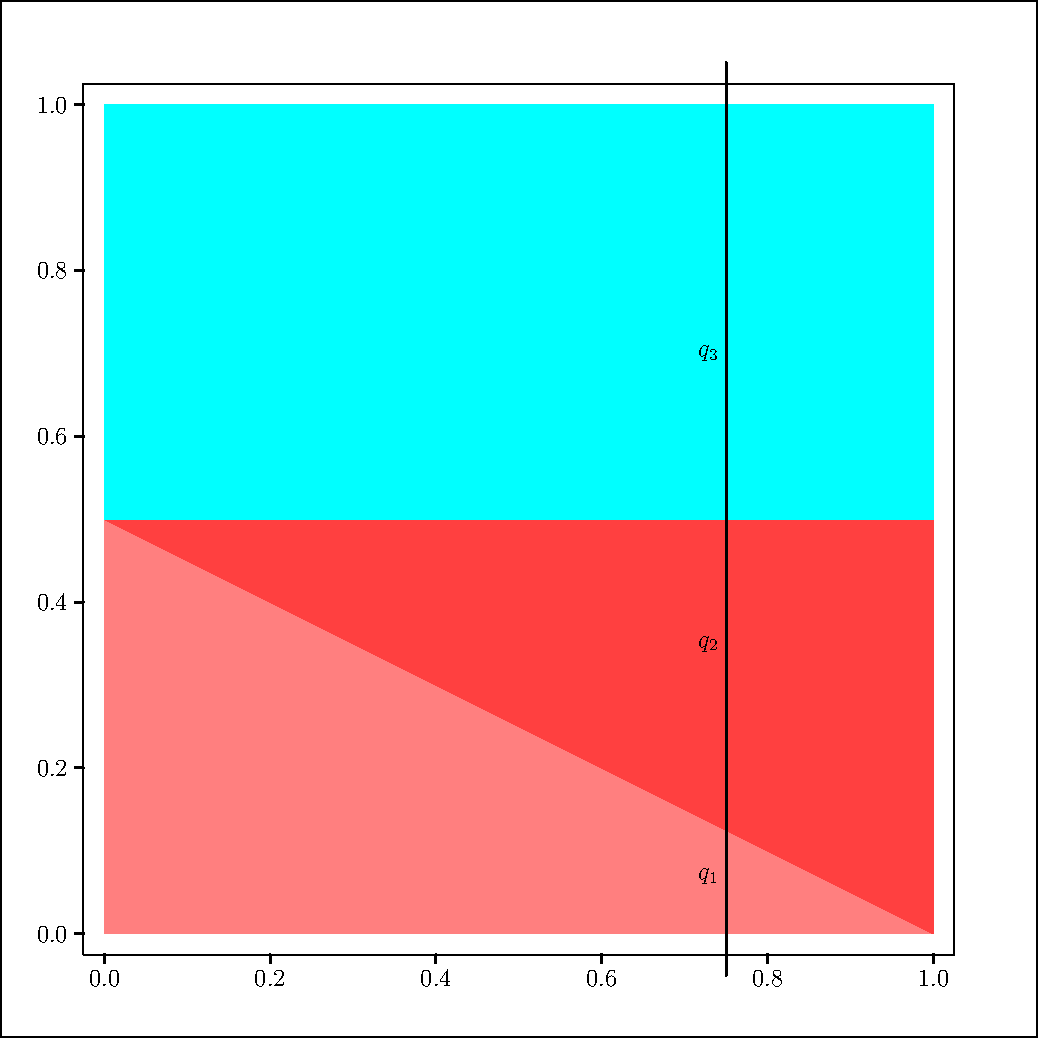
\includegraphics[width=\textwidth]{zeroone-unif.pdf}
      \caption{Judy Benjamin's updated probability assignment
        according to intuition T1. $0<q<1$ forms the horizontal axis,
        the vertical axis shows the updated probability distribution
        (or the normalized odds vector) $(q_{1},q_{2},q_{3})$. The
        vertical line at $q=0.75$ shows the specific updated
        probability distribution $G_{\mbox{\tiny ind}}(0.75)$ for the Judy
        Benjamin problem.}
      \label{fig:unif}
    \end{minipage}
  \end{flushright}
\end{figure}

\begin{figure}[h]
  \begin{flushright}
    \begin{minipage}[h]{\lwv\linewidth}
      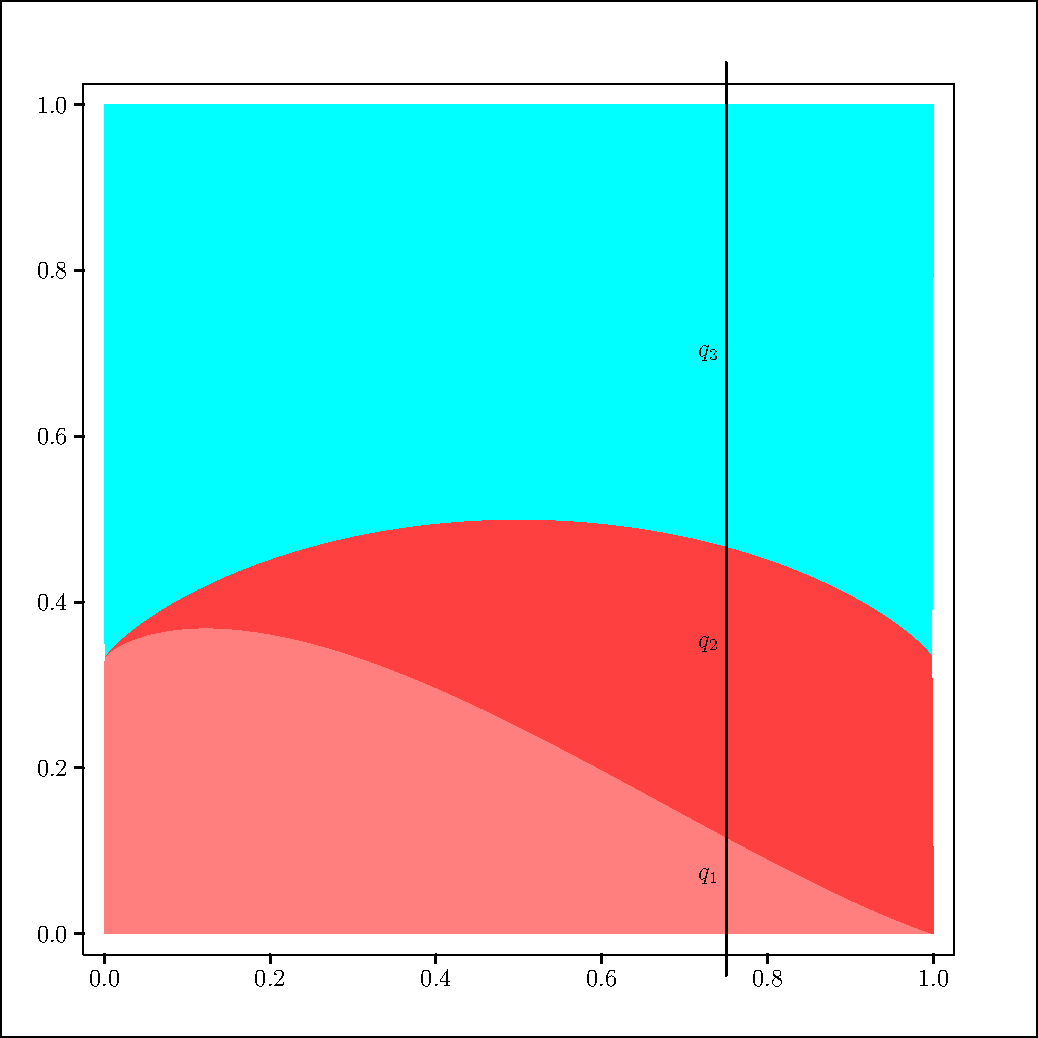
\includegraphics[width=\textwidth]{zeroone-mxnt.pdf}
      \caption{Judy Benjamin's updated probability assignment using
        \textsc{maxent}. $0<q<1$ forms the horizontal axis, the
        vertical axis shows the updated probability distribution (or
        the normalized odds vector) $(q_{1},q_{2},q_{3})$. The
        vertical line at $q=0.75$ shows the specific updated
        probability distribution $G_{\mbox{\tiny max}}(0.75)$ for the Judy
        Benjamin problem.}
      \label{fig:mxnt}
    \end{minipage}
  \end{flushright}
\end{figure}

\medskip

\kapt{Epistemic Entrenchment and Coarsening at Random}

\smallskip

\nias Even though T1 is an understandably strong intuition, it does
not take into account that the information given to Judy by her
commanders may be dependent on whether she is in Blue or in Red
territory. To underline this objection to intuition T1 we want to
consider three scenarios, any of which may form the basis of the
partial information provided by her commanders.

\begin{enumerate}
\item[\textbf{I}] Judy is dropped off by a pilot who flips two
  coins. If the first coin lands H, then Judy is dropped off in Blue
  territory, otherwise in Red territory. If the second coin lands H,
  she is dropped off in the Headquarters area, otherwise in the
  Second Company area. Judy's commanders find out that the second coin
  is biased $q:1-q$ toward H with $q=0.75$. The normalized odds
  vector is $G_{\mbox{\tiny I}}(0.75)=(0.125,0.375,0.500)$ and agrees
  with T1, because the choice of Blue or Red is completely independent
  from the choice of the Red Headquarters area or the Red Second
  Company area.
\item[\textbf{II}] The pilot randomly lands in any of the four
  quadrants and rolls a die. If she rolls an even number, she drops
  off Judy. If not, she takes her to another (or the same, the choice
  happens with replacement) randomly selected quadrant to repeat the
  procedure. Judy's commanders find out, however, that for $A_{1}$,
  the pilot requires a six to drop off Judy, not just an even number.
  The normalized odds vector in this scenario is $G_{\mbox{\tiny
      II}}(0.75)=(0.1,0.3,0.6)$ and does not accord with T1.
\item[\textbf{III}] Judy's commanders have divided the map into $24$
  congruent rectangles, $A_{3}$ into twelve, and $A_{1}$ and $A_{2}$
  into six rectangles each (see figures~\ref{fig:pwstex1} and
  \ref{fig:pwstex2}). They have information that the only subsets of
  the $24$ rectangles in which Judy Benjamin may be located are such
  that they contain three times as many $A_{2}$ rectangles than
  $A_{1}$ rectangles. The normalized odds vector in this scenario is
  $G_{\mbox{\tiny III}}(0.75)\approx(.108,.324,.568)$ (evaluating almost
  17 million subsets).
\end{enumerate}

I--III demonstrate the contrast between scenarios when independence is
true and when it is not. Douven and Romeijn's capital mistake in their
paper is that they assume that the Judy Benjamin problem is analogous
to their example of Sarah and the sundowners at the Westcliff (see
\scite{8}{douvenromeijn09}{7}). Sarah, however, knows that whether it
rains or not is independent of her activity the next night, whereas in
Judy Benjamin we have no evidence of such independence, as scenario II
demonstrates. Douven and Romeijn's reliance on intuition T1 leads them
to apply Jeffrey's rule to the Judy Benjamin problem with the
additional constraint $q_{3}=p_{3}$. They claim that in most cases
\qeins{the learning of a conditional is or would be irrelevant to
  one's degree of belief for the conditional's antecedent {\ldots} the
  learning of the relevant conditional should intuitively leave the
  probability of the antecedent unaltered}
\scite{2}{douvenromeijn09}{9}.

This, according to Douven and Romeijn, is the usual epistemic
entrenchment and applies in full force to the Judy Benjamin problem.
They give an example where the epistemic entrenchment could go the
other way and leave the consequent rather than the antecedent
unaltered (Kate and Henry, see \scite{8}{douvenromeijn09}{13}). The
idea of epistemic entrenchment is at odds with \textsc{maxent} and
seems to imply just what the full employment theorem claims: judgments
so framed \qeins{will depend on the judgmental skills of the agent,
  typically acquired not in the inductive logic class but by subject
  specific training} \scite{2}{bradley05}{349}. To pursue the
relations between epistemic entrenchment, \textsc{maxent}, and the
full employment theorem would take us too far afield at present and
shall be undertaken elsewhere. For the Judy Benjamin problem, it is
not clear why Douven and Romeijn think that the way the problem is
posed implies a strong epistemic entrenchment for Adams conditioning
(Adams conditioning is the kind of conditioning that will leave the
antecedent alone). Scenarios II-III provide realistic alternatives
where Adams conditioning is inappropriate. 

Judy Benjamin may also receive ({\ref{eq:hdq}}) because her informers
have found out that Red Headquarters troops have occupied the entire
Blue territory ($q_{1}=3p_{1},q_{2}=p_{2},q_{3}=0$, the epistemic
entrenchment is with respect to $q_{2}$); because they have found out
that Blue troops have occupied two-thirds of the Red Second Company
area ($q_{1}=p_{1},q_{2}=(1/3)p_{2},q_{3}=(4/3)p_{3}$, the epistemic
entrenchment is with respect to $q_{1}$); or because they have found
out that Red Headquarters troops have taken over half of the Red
Second Company area ($q_{1}=(1/2)p_{1},q_{2}=(3/2)p_{2},q_{3}=p_{3}$,
the epistemic entrenchment is with respect to $q_{3}$ and what Douven
and Romeijn take to be an assumption in the wording of the problem).
There is nothing in the problem that supports Douven and Romeijn's
narrowing of the options. The table reiterates these options, with the
third, shaded line representing intuition (T1) and the epistemic
entrenchment defended by Douven and Romeijn.

\rowcolors{4}{lightgray}{lightgray}
\begin{tabular}{|l|c|c|c|}\hline
Epistemic entrenchment & $q_{1}$ & $q_{2}$ & $q_{3}$ \\ \hline
with respect to $A_{1}$ & 1/4 & 3/4 & 0 \\ \hline
with respect to $A_{2}$ & 1/12 & 1/4 & 2/3 \\ \hline
with respect to $A_{3}$ & 1/8 & 3/8 & 1/2 \\ \hline
\end{tabular}

\bigskip

\bigskip

\nias Another at first blush forceful argument that \textsc{maxent}'s
solution for the Judy Benjamin problem is counterintuitive has to do
with coarsening at random, or CAR for short. It is spelled out in
Gr{\"u}nwald and Halpern (2003)\nonsc{}. Gr{\"u}nwald and Halpern see
a parallel between the Judy Benjamin problem and Martin Gardner's
Three Prisoners problem (see \scite{8}{gardner59}{180f}). In the Three
Prisoners problem, three men (A, B, and C) are under sentence of death
when the governor decides to pardon one of them. The warden of the
prison knows which of the three men is pardoned, but none of the men
do. In a private conversation, A says to the warden, Tell me the name
of one of the others who will be executed---it will not give anything
away whether I will be executed or not. The warden agrees and tells A
that B will be executed. For the puzzling consequences, see the wealth
of literature on the Three Prisoners problem or the Monty Hall
problem.

According to Gr{\"u}nwald and Halpern, for problems of this kind (Judy
Benjamin, Three Prisoners, Monty Hall) there are naive and
sophisticated spaces to which we can apply probability updates. If A
uses the naive space, for example, he comes to the following
conclusion: of the three possibilities that (A,B), (A,C), or (B,C) are
executed, the warden's information excludes (A,C). (A,B) and (B,C) are
left over, and because A has no information about which one of these
is true his chance of not being executed is 0.5. His chance of
survival has increased from one third to one half. 

Gr{\"u}nwald and Halpern show, correctly, that the application of the
naive space is illegitimate because the CAR condition does not hold.
More generally, Gr{\"u}nwald and Halpern show that updating on the
naive space rather than the sophisticated space is legitimate for
event type observations always when the set of observations is
pairwise disjoint or, when the events are arbitrary, only when the CAR
condition holds. For Jeffrey type observations, there is a generalized
CAR condition which applies likewise. For affine constraints on which
we cannot use Jeffrey conditioning (or, a fortiori, standard
conditioning) \textsc{maxent }\qeins{essentially never gives the right
  results} \scite{2}{gruenwaldhalpern03}{243}.

Gr{\"u}nwald and Halpern conclude that \qeins{working with the naive
  space, while an attractive approach, is likely to give highly
  misleading answers} (246), especially in the application of
\textsc{maxent} to naive spaces as in the Judy Benjamin case
\qeins{where applying [\textsc{maxent}] leads to paradoxical, highly
  counterintuitive results} (245). For the Three Prisoners problem,
Jaynes' constraint rule would supposedly proceed as follows: the
vector of prior probabilities for (A,B), (A,C), and (B,C) is
$(1/3,1/3,1/3)$. The constraint is that the probability of (A,C) is
zero, and a simple application of the constraint rule yields
$(1/2,0,1/2)$ for the vector of updated probabilities. The CAR
condition for the naive space does not hold, therefore the result is
misleading.

By analogy, using the constraint rule on the naive space for the Judy
Benjamin problem yields $(0.117,0.350,0.533)$, but as the CAR
condition fails in even the simplest settings for affine constraints
(\qeins{CAR is (roughly speaking) guaranteed \emph{not} to hold except
  in \qzwei{degenerate} situations} (251), emphasis in the original),
it certainly fails for the Judy Benjamin problem, for which
constructing a sophisticated space is complicated (see
\scite{7}{grovehalpern97}{}, where the authors attempt such a
construction by retrospective conditioning).

The analogy, however, is misguided. The constraint rule has been
formally shown to generalize Jeffrey conditioning, which in turn has
been shown to generalize standard conditioning (the authors admit as
much in \scite{8}{gruenwaldhalpern03}{262}). We can solve both the
Monty Hall problem and the Three Prisoners problem by standard
conditioning, not using the naive space, but simply using the correct
space for the probability update. For the Three Prisoners problem, for
example, the warden will say either \qnull{B} or \qnull{C} in response
to A's inquiry. Because A has no information that would privilege
either answer the probability that the warden says \qnull{B} and the
probability that the warden says \qnull{C} equal each other and
therefore equal 0.5. Here is the difference between using the naive
space and using the correct space, but either way using standard
conditional probabilities:
%  ($P'$ is the prior
% probability, before A receives the warden's information, $P''$ is the
% updated probability):

\begin{displaymath}
  P(\mbox{`A is pardoned'}|\mbox{`B will be
    executed'})=
\end{displaymath}
\begin{displaymath}
  \frac{P(\mbox{`A is pardoned'})}{P(\mbox{`A is
      pardoned'})+P(\mbox{`C is pardoned'})}=\frac{1}{2}\mbox{ (incorrect)}
\end{displaymath}

\begin{displaymath}
  P(\mbox{`A is pardoned'}|\mbox{`warden says B will be
    executed'})=
\end{displaymath}
\begin{displaymath}
  \frac{P(\mbox{`A is pardoned' and `warden says B will
      be executed'})}{P(\mbox{`warden says B will be
      executed'})}=\frac{1/6}{1/2}=\frac{1}{3}\mbox{ (correct)}
\end{displaymath}

\nial Why is the first equation incorrect and the second one correct?
Information theory gives us the right answer: in the first equation,
we are conditioning on a watered down version of the evidence (watered
down in a way that distorts the probabilities because we are not
\qnull{coarsening at random}). \qnull{Warden says B will be executed}
is sufficient but not necessary for \qnull{B will be executed.} The
former proposition is more informative than the latter proposition
(its probability is lower). Conditioning on the latter proposition
leaves out relevant information contained in the wording of the
problem.

Because \textsc{maxent} always agrees with standard conditioning,
\textsc{maxent} gives the correct result for the Three Prisoners
problem. For the Judy Benjamin problem, there is no defensible
sophisticated space and no watering down of the evidence in what
Gr{\"u}nwald and Halpern call the \qnull{naive} space. The analogy
between the Three Prisoners problem and the Judy Benjamin problem as
it is set up by Gr{\"u}nwald and Halpern fails. A successful criticism
would be directed at the construction of the \qnull{naive} space: this
is what we just accomplished for the Three Prisoners problem. There is
no parallel procedure for the Judy Benjamin problem. The \qnull{naive}
space is all we have, and \textsc{maxent} is the appropriate tool to
deal with this lack of information.

\medskip

\kapt{The Powerset Approach}

\smallskip

\nias In this section, we will focus on scenario III and consider what
happens when the grain of the partition becomes finer. We call this
the powerset approach. Two remarks are in order: First, the powerset
approach has little independent appeal. The reason behind using
\textsc{maxent} is that we want our evidence to have just the right
influence on our updated probabilities, i.e.\ neither over-inform
nor under-inform. There is no corresponding reason why we should
update our probabilities using the powerset approach.

Second, what the powerset approach does is lend support to another
approach. In this task, it is persuasive because it tells us what
would happen if we were to divide the event space into infinitesimally
small, uniformly weighed, and independent \qnull{atomic} bits of
information. It would be especially interesting if the powerset
approach did not support the independence and uniformity assumptions
of intuition T1, because both of these features are strongly
represented in the powerset approach. On its own the powerset approach
is just what Gr{\"u}nwald and Halpern call a naive space, for which
CAR does not hold. Hence the powerset approach will not give us a
precise solution for the problem, although it may with some
plausibility guide us in the right direction---especially if despite
all its independence and uniformity assumptions it significantly
disagrees with intuition T1.

% Let's assume a partition $\{B_{i}\}_{i=1,{\ldots},4n}$ of
% $A_{1}\cup{}A_{2}\cup{}A_{3}$ into sets that are of equal measure
% $\mu$ and whose intersection with $A_{i}$ is either the empty set or
% the whole set itself (this is the division into rectangles of scenario
% III). ({\ref{eq:map}}) dictates that the number of sets covering $A_{3}$ equals
% the number of sets covering $A_{1}\cup{}A_{2}$. For convenience, we
% assume the number of sets covering $A_{1}$ to be $n$. Let
% $\mathcal{C}$, a subset of the powerset of
% $\{B_{i}\}_{i=1,{\ldots},4n}$, be the collection of sets which agree
% with the constraint imposed by ({\ref{eq:hdq}}), i.e.\
% \begin{displaymath}
%   C\in\mathcal{C}\mbox{ iff }C=\{C_{j}\}\mbox{ and }t\mu\left(\bigcup{}C_{j}\cap{}A_{1}\right)=\mu\left(\bigcup{}C_{j}\cap{}A_{2}\right)
% \end{displaymath}
% In figures~\ref{fig:pwstex1} and \ref{fig:pwstex2} there are diagrams
% of two elements of the powerset of $\{B_{i}\}_{i=1,{\ldots},4n}$. One
% of them (figure~\ref{fig:pwstex1}) is not a member of $\mathcal{C}$,
% the other one (figure~\ref{fig:pwstex2}) is. 

Let's assume a partition of the Blue and Red territories into sets of
equal measure (this is the division into rectangles of scenario III).
({\ref{eq:map}}) dictates that the number of sets covering $A_{3}$
equals the number of sets covering $A_{1}\cup{}A_{2}$. Initially, any
subset of this partition is a candidate for Judy Benjamin to consider.
The constraint imposed by ({\ref{eq:hdq}}) is that now we only
consider subsets for which there are three times as many partition
sets (or rectangles, although we are not necessarily limiting
ourselves to rectangles) in $A_{2}$ than there are in $A_{1}$. In
figures~\ref{fig:pwstex1} and \ref{fig:pwstex2} there are diagrams of
two subsets. One of them (figure~\ref{fig:pwstex1}) is not a
candidate, the other one (figure~\ref{fig:pwstex2}) is.

\begin{figure}[h]
  \begin{flushright}
    \begin{minipage}[h]{\lwv\linewidth}
      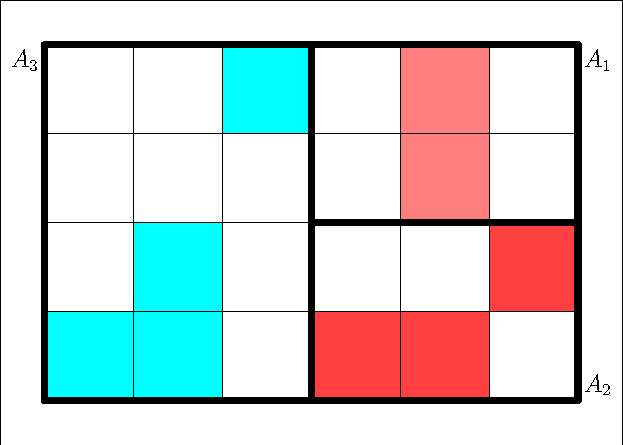
\includegraphics[width=\textwidth]{partition-2.pdf}
      \caption{This choice of rectangles is not a candidate because
        the number of rectangles in $A_{2}$ is not a $t$-multiple of
        the number of rectangles in $A_{1}$, here with $s=2,t=3$ as in
        scenario III.}
      \label{fig:pwstex1}
    \end{minipage}
  \end{flushright}
\end{figure}

\begin{figure}[h]
  \begin{flushright}
    \begin{minipage}[h]{\lwv\linewidth}
      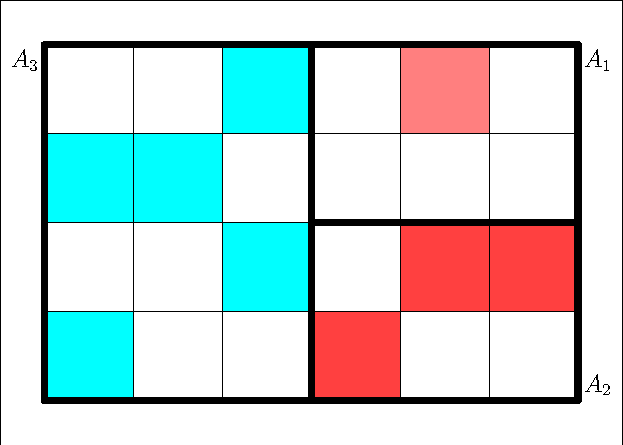
\includegraphics[width=\textwidth]{partition-1.pdf}
      \caption{This choice of rectangles is a candidate because the
        number of rectangles in $A_{2}$ is a $t$-multiple of the
        number of rectangles in $A_{1}$, here with $s=2,t=3$ as in
        scenario III.}
      \label{fig:pwstex2}
    \end{minipage}
  \end{flushright}
\end{figure}

Let $X$ be the random variable that corresponds to the ratio of the
number of partition elements (rectangles) that are in $A_{3}$ and the
total number of partition elements (rectangles) for a randomly chosen
candidate. We would now anticipate that the expectation of $X$ (which
we will call $EX$) gives us an indication of the updated probability
that Judy is in $A_{3}$ (so $EX\approx{}q_{3}$). The powerset approach
is often superior to the uniformity approach (Grove and Halpern use
uniformity, with all the necessary qualifications): if you have played
Monopoly, you will know that the frequencies for rolling a 2, a 7, or
a 10 with two dice tend to conform more closely to the binomial
distribution (based on a powerset approach) rather than to the uniform
distribution with $P(\mbox{rolling }i)=1/11$ for $i=2,{\ldots},12$.

% Appendix II provides a formula for the powerset approach corresponding
% to the formula for the \textsc{maxent} approach, giving us $q_{3}$
% dependent on $t$. Notice that this formula is for $t=2,3,4,\ldots$.
% For $t=1$ use the Chu-Vandermonde identity to find that
% \begin{displaymath}
%   EX_{12}=(t+1)\frac{\sum_{i=1}^{s}i\binom{ts}{i}\binom{ts}{ti}}{\sum_{i=0}^{s}\binom{ts}{i}\binom{ts}{ti}}=(t+1)\frac{s}{2}  
% \end{displaymath}
% and consequently $EX=1/2$, as one would expect. For
% $t=1/2,1/3,1/4,\ldots$ we can simply reverse the roles of $A_{1}$ and
% $A_{2}$. These results 

Calculations not provided here give us $G_{\mbox{\tiny pws}}$ and a
graph of the normalized odds vector (see figure~\ref{fig:pwst}), a bit
bumpy around the middle because the $t$-values are discrete and
farther apart in the middle, as $t=q/(1-q)$. Comparing the graphs of
the normalized odds vector under Grove and Halpern's uniformity
approach ($G_{\mbox{\tiny ind}}$), Jaynes' \textsc{maxent} approach
($G_{\mbox{\tiny max}}$), and the powerset approach suggested in this
paper ($G_{\mbox{\tiny pws}}$), it is clear that the powerset approach
supports \textsc{maxent}.

\begin{figure}[h]
  \begin{flushright}
    \begin{minipage}[h]{\lwv\linewidth}
      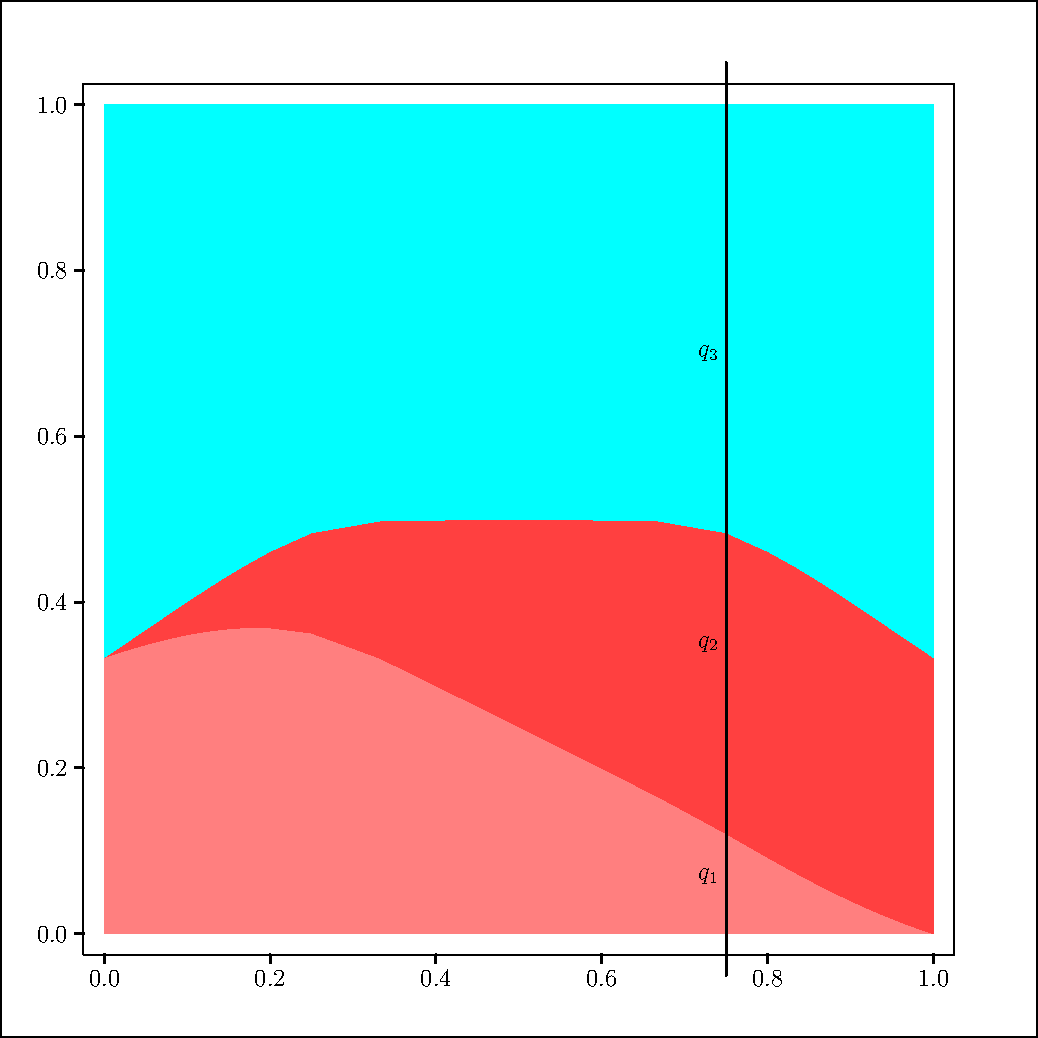
\includegraphics[width=\textwidth]{zeroone-pwst.pdf}
      \caption{Judy Benjamin's updated probability assignment
        according to the powerset approach. $0<q<1$ forms the
        horizontal axis, the vertical axis shows the updated
        probability distribution (or the normalized odds vector)
        $(q_{1},q_{2},q_{3})$. The vertical line at $q=0.75$ shows the
        specific updated probability distribution $G_{\mbox{\tiny
            pws}}$ for the Judy Benjamin problem.}
      \label{fig:pwst}
    \end{minipage}
  \end{flushright}
\end{figure}

Going through the calculations, it seems at many places that the
powerset approach should give its support to Grove and Halpern's
uniformity approach in keeping with intuition T1. It is unexpected to
% find out that in the mathematical analysis $\alpha_{t,s}$ converges to
find out that in the mathematical analysis the parameters converge to
a non-trivial factor and do not tend to negative or positive infinity,
enabling a graph of the normalized odds vector that is not of the
simple nature of the graph suggested by Grove and Halpern. Most
surprisingly, the powerset approach, prima facie unrelated to an
approach using information, supports the idea that a set of events
about which nothing is known (such as $A_{3}$) gains in probability in
the updated probability distribution compared to the set of events
about which something is known (such as $A_{1}$ and $A_{2}$), even if
it is only partial information. Unless independence is specified, as
in Sarah and sundowners at the Westcliff, the area of ignorance gains
compared to the area of knowledge.

We now have several ways to characterize Judy's updated
probabilities and updated probabilities following upon partial
information in general. Only one of them, the uniformity approach,
violates van Fraassen, Hughes, and Harman's five symmetry requirements
in \scite{1}{fraassenetal86}{} and intuition T2. The uniformity
approach, however, is the only one that satisfies intuition T1, an
intuition which most people have when they first hear the story. Two
arguments attenuate the position of the uniformity approach in
comparison with the others. 

First, T1 rests on an independence assumption which is not reflected
in the problem. Although there is no indication that what Judy's
commanders tell her is in any way dependent on her probability of
being in Blue territory, it is not excluded either (see scenarios
I--III earlier in this paper). \textsc{maxent} takes this uncertainty
into consideration. Second, when we investigate the problem using the
powerset approach it turns out that a division into equally probable,
independent, and increasingly fine bits of information supports not
intuition T1 but rather intuition T2. \textsc{maxent}, for now, is
vindicated. We need to look for full employment not by looking at
cleverly manipulating prior probabilities, but by making fresh
observations, designing better experiments, and partitioning the
theory space more finely.

% \newpage

% \kapt{Appendix I}

% \nias Appendix I provides a concise but comprehensive summary of
% Jaynes' constraint rule not easily obtainable in the literature.
% Jaynes applied it to the Brandeis Dice Problem (see
% \scite{8}{jaynes89}{243}), but does not give a mathematical
% justification.

% Let $f$ be a probability distribution on a finite space
% $x_{1},\ldots,x_{m}$ that fulfills the constraint 
% \begin{equation}
%   \label{eq:constraint}
% \sum_{i=1}^{m}r(x_{i})f(x_{i})=\alpha
% \end{equation}

% An affine constraint can always be expressed by assigning a value to
% the expectation of a probability distribution (see
% \scite{7}{hobson71}{}). In Judy Benjamin's case, for example, let
% $r(x_{1})=0, r(x_{2})=1, r(x_{3})=q\mbox{ and }\alpha=q$. Because $f$
% is a probability distribution it fulfills
% \begin{equation}
%   \label{eq:unity}
% \sum_{i=1}^{m}f(x_{i})=1
% \end{equation}

% We want to maximize Shannon's entropy, given the constraints
% ({\ref{eq:constraint}}) and ({\ref{eq:unity}}),
% \begin{equation}
%   \label{eq:entropy}
% -\sum_{i=1}^{m}f(x_{i})\ln(x_{i})
% \end{equation}

% We use Lagrange multipliers to define the functional
% \begin{equation}
%   \label{eq:functional}
% J(f)=-\sum_{i=1}^{m}f(x_{i})\ln{}f(x_{i})+\lambda_{0}\sum_{i=1}^{m}f(x_{i})+\lambda_{1}\sum_{i=1}^{m}r(x_{i})f(x_{i})\notag
% \end{equation}
% and differentiate it with respect to $f(x_{i})$
% \begin{equation}
%   \label{eq:funder}
% \frac{\partial{}J}{\partial{}f(x_{i})}=-\ln(f(x_{i}))-1+\lambda_{0}+\lambda_{1}r(x_{i})
% \end{equation}

% Set ({\ref{eq:funder}}) to $0$ to find the necessary condition to
% maximize ({\ref{eq:entropy}})
% \begin{equation}
%   \label{eq:coverthomas}
% g(x_{i})=e^{\lambda_{0}-1+\lambda_{1}r(x_{i})}\notag
% \end{equation}

% This is the Gibbs distribution. We still need to do two things: (a)
% show that the entropy of $g$ is maximal, and (b) show how to find
% $\lambda_{0}$ and $\lambda_{1}$. (a) is shown in Theorem 12.1.1 in
% Cover and Thomas \scite{1}{coverthomas06}{} and there is no reason to
% copy it here. 

% For (b), let
% \begin{equation}
%   \label{eq:l1}
% \lambda_{1}=-\beta\notag
% \end{equation}
% \begin{equation}
%   \label{eq:zet}
% Z(\beta)=\sum_{i=1}^{m}e^{-\beta{}r(x_{i})}\notag
% \end{equation}
% \begin{equation}
%   \label{eq:l0}
% \lambda_{0}=1-\ln(Z(\beta))\notag
% \end{equation}

% To find $\lambda_{0}$ and $\lambda_{1}$ we introduce the constraint
% \begin{equation}
%   \label{eq:logcon}
% -\frac{\partial}{\partial{}\beta}\ln(Z(\beta))=\alpha\notag
% \end{equation}

% To see how this constraint gives us $\lambda_{0}$ and $\lambda_{1}$,
% Jaynes' solution of the Brandeis Dice Problem (see
% \scite{8}{jaynes89}{243}) is a helpful example. We are, however,
% interested in a general proof that this choice of $\lambda_{0}$ and
% $\lambda_{1}$ gives us the probability distribution maximizing the
% entropy. That $g$ so defined maximizes the entropy is shown in (a). We
% need to make sure, however, that with this choice of $\lambda_{0}$ and
% $\lambda_{1}$ the constraints ({\ref{eq:constraint}}) and
% ({\ref{eq:unity}}) are also fulfilled.

% First, we show
% % \begin{align}
% % &\mathbb{R}^{3}\mbox{ can be endowed with a metric }l_{2}\notag
% % \\
% % &\mbox{with constant positive curvature }K=k\label{carmor2}\tag{C2}
% % \end{align}
% \begin{align}
% &\sum_{i=1}^{m}g(x_{i})=\sum_{i=1}^{m}e^{\lambda_{0}-1+\lambda_{1}r(x_{i})}=e^{\lambda_{0}-1}\sum_{i=1}^{m}e^{\lambda_{1}r(x_{i})}=\notag\\
% &e^{-\ln(Z(\beta))}Z(\beta)=1\label{eq:unishow}\notag
% \end{align}

% Then, we show, by differentiating $\ln(Z(\beta))$ using the
% substitution $x=e^{-\beta}$
% \begin{align}
% &\alpha=-\frac{\partial}{\partial{}\beta}\ln(Z(\beta))=-\frac{1}{\sum_{i=1}^{m}x^{r(x_{i})}}\left(\sum_{i=1}^{m}r(x_{i})x^{r(x_{i})-1}\right)(-x)=\notag\\
% &\frac{\sum_{i=1}^{m}r(x_{i})x^{r(x_{i})}}{\sum_{i=1}^{m}x^{r(x_{i})}}\notag
% \end{align}

% And, finally,
% \begin{align}
% &\sum_{i=1}^{m}r(x_{i})g(x_{i})=\sum_{i=1}^{m}r(x_{i})e^{\lambda_{0}-1+\lambda_{1}r(x_{1})}=e^{\lambda_{0}-1}\sum_{i=1}^{m}r(x_{i})e^{\lambda_{1}r(x_{1})}=\notag\\
% &e^{\lambda_{0}-1}\sum_{i=1}^{m}r(x_{i})x^{r(x_{i})}=\alpha{}e^{\lambda_{0}-1}\sum_{i=1}^{m}x^{r(x_{i})}=\alpha{}e^{\lambda_{0}-1}\sum_{i=1}^{m}e^{-\beta{}r(x_{i})}=\notag\\
% &\alpha{}Z(\beta)e^{\lambda_{0}-1}=\alpha{}Z(\beta))e^{-\ln(Z(\beta))}=\alpha\notag
% \end{align}

% Filling in the variables from Judy Benjamin's scenario gives us result
% ({\ref{eq:vmax}}). The lambdas are:
%   \begin{displaymath}
%     \lambda_{0}=1-\ln\left(\sum_{i=1}^{m}e^{\lambda_{1}r(x_{i})}\right)\hspace{.3in}
%     \lambda_{1}=\ln{}q-\ln(1-q)\notag
%   \end{displaymath}

%   We combine the normalized odds vector $(0.16,0.48,0.36)$ following
%   from these lambdas using Dempster's Rule of Combination with
%   ({\ref{eq:map}}) and get result ({\ref{eq:vmax}}).

% \medskip

% \kapt{Appendix II}

% \nias The binomial distribution dictates the value of $EX$, using
% simple combinatorics. In this case we require, again for convenience,
% that $n$ be divisible by $t$ and the \qnull{grain} of the partition
% $A$ be $s=n/t$. We introduce a few variables which later on will help
% for abbreviation:
% \begin{displaymath}
% n=ts\hspace{.5in}
% 2m=n\hspace{.5in}
% 2j=n-1\hspace{.5in}
% {T}=t^{2}+1
% \end{displaymath}
% $EX$, of course, depends both on the grain of $A$ and the value of
% $t$. It makes sense to make it independent of the grain by letting the
% grain become increasingly finer and by determining $EX$ as
% $s\rightarrow\infty$. This cannot be done for the binomial
% distribution, as it is notoriously uncomputable for large numbers
% (even with a powerful computer things get dicey around $s=10$). But,
% equally notorious, the normal distribution provides a good
% approximation of the binomial distribution and will help us arrive at
% a formula for $G_{\mbox{\tiny pws}}$ (corresponding to 
% $G_{\mbox{\tiny ind}}$ and $G_{\mbox{\tiny max}}$), determining the value $q_{3}$
% dependent on $q$ as suggested by the powerset approach.

% First, we express the random variable $X$ by the two independent
% random variables $X_{12}$ and $X_{3}$. $X_{12}$ is the number of
% partition elements in the randomly chosen $C$ which are either in
% $A_{1}$ or in $A_{2}$ (the random variable of the number of partition
% elements in $A_{1}$ and the random variable of the number of partition
% elements in $A_{2}$ are decisively not independent, because they need
% to obey ({\ref{eq:hdq}})); $X_{3}$ is the number of partition elements
% in the randomly chosen $C$ which are in $A_{3}$. A relatively simple
% calculation shows that $EX_{3}=n$, which is just what we would expect
% (either the powerset approach or the uniformity approach would give us
% this result):
% \begin{displaymath}
%   EX_{3}=2^{-2n}\sum_{i=0}^{2n}i\binom{2n}{i}=n\mbox{ (use }\binom{n}{k}=\frac{n}{k}\binom{n-1}{k-1}\mbox{)}
% \end{displaymath}

% The expectation of $X$, $X$ being the random variable expressing the
% ratio of the number of sets covering $A_{3}$ and the number of sets
% covering $A_{1}\cup{}A_{2}\cup{}A_{3}$, is
% \begin{displaymath}
%   EX=\frac{EX_{3}}{EX_{12}+EX_{3}}=\frac{n}{EX_{12}+n}
% \end{displaymath}
% If we were able to use uniformity and independence, $EX_{12}=n$ and
% $EX=1/2$, just as Grove and Halpern suggest (although their uniformity
% approach is admittedly less crude than the one used here). Will the
% powerset approach concur with the uniformity approach, will it support
% the principle of maximum entropy, or will it make another suggestion
% on how to update the prior probabilities? To answer this question, we
% must find out what $EX_{12}$ is, for a given value $t$ and
% $s\rightarrow\infty$, using the binomial distribution and its
% approximation by the normal distribution.

% Using combinatorics,
% \begin{displaymath}
%   EX_{12}=(t+1)\frac{\sum_{i=1}^{s}i\binom{ts}{i}\binom{ts}{ti}}{\sum_{i=0}^{s}\binom{ts}{i}\binom{ts}{ti}}
% \end{displaymath}

% Let us call the numerator of this fraction NUM and the denominator
% DEN. According to the de Moivre-Laplace Theorem,
% \begin{displaymath}
%   \mbox{DEN}=\sum_{i=0}^{s}\binom{ts}{i}\binom{ts}{ti}\approx{}2^{2n}\sum_{i=0}^{s}\int_{i-\frac{1}{2}}^{i+\frac{1}{2}}\mathcal{N}(\frac{n}{2},\frac{n}{4})(i)\mathcal{N}(\frac{n}{2},\frac{n}{4})(ti)di
% \end{displaymath}
% where
% \begin{displaymath}
%   \mathcal{N}(\mu,\sigma^{2})(x)=\frac{1}{\sqrt{2\pi\sigma^{2}}}\exp\left(-\frac{(x-\mu)^{2}}{2\sigma^{2}}\right)
% \end{displaymath}
% Substitution yields
% \begin{displaymath}
%   \mbox{DEN}\approx{}2^{2n}\frac{1}{\pi{}m}\sum_{i=0}^{s}\int_{i-\frac{1}{2}}^{i+\frac{1}{2}}\exp\left(-\frac{\left(x-m\right)^{2}}{m}-\frac{t^{2}\left(x-\frac{m}{t}\right)^{2}}{m}\right)dx
% \end{displaymath}
% Consider briefly the argument of the exponential function:
% \begin{displaymath}
%   -\frac{\left(x-m\right)^{2}}{m}-\frac{t^{2}\left(x-\frac{m}{t}\right)^{2}}{m}=-\frac{t^{2}}{m}({\aden}x^{2}+{\bden}x+{\cden})=-\frac{t^{2}}{m}\left({\aden}(x-{\hden})^{2}+{\kden}\right)
% \end{displaymath}
% with (the double prime sign corresponds to the simple prime sign for
% the numerator later on)
% \begin{displaymath}
% {\aden}=\frac{1}{t^{2}}{T}\notag\hspace{.5in}
% {\bden}=(-2m)\frac{1}{t^{2}}(t+1)\hspace{.5in}
% {\cden}=2m^{2}\frac{1}{t^{2}}
% \end{displaymath}
% \begin{displaymath}
% {\hden}=-{\bden}/2{\aden}\hspace{.5in}
% {\kden}={\aden}{\hden}^{2}+{\bden}{\hden}+{\cden}
% \end{displaymath}
% Consequently,
% \begin{displaymath}
% \mbox{DEN}\approx{}2^{2n}\exp\left(-\frac{t^{2}}{m}{\kden}\right)\sqrt{\frac{1}{\pi{}{\aden}mt^{2}}}\int_{-\infty}^{s+\frac{1}{2}}\mathcal{N}\left({\hden},\frac{m}{2{\aden}t^{2}}\right)dx
% \end{displaymath}
% And, using the error function for the cumulative density function of
% the normal distribution,
% \begin{equation}
%   \label{eq:den}
%   \mbox{DEN}\approx{}2^{2n-1}\sqrt{\frac{1}{\pi{}{\aden}mt^{2}}}\exp\left(-\frac{{\kden}t^{2}}{m}\right)\left(1-\erf({\wden})\right)
% \end{equation}
% with
% \begin{displaymath}
%   {\wden}=\frac{t\sqrt{{\aden}}\left(s+\frac{1}{2}-{\hden}\right)}{\sqrt{m}}
% \end{displaymath}

% We proceed likewise with the numerator, although the additional factor
% introduces a small complication:
%   \begin{eqnarray*}
%   \mbox{NUM}&=&\sum_{i=1}^{s}i\binom{ts}{i}\binom{ts}{ti}=\sum_{i=1}^{s}s\binom{ts}{i}\binom{ts-1}{ti-1}\\
% &\approx&s2^{2n-1}\sum_{i=1}^{s}\mathcal{N}\left(m,\frac{m}{2}\right)(i)\mathcal{N}\left(j,\frac{j}{2}\right)(ti-1)
% \end{eqnarray*}
% Again, we substitute and get
% \begin{displaymath}
%   \mbox{NUM}\approx{}s2^{2n-1}\left(\pi\sqrt{mj}\right)^{-1}\sum_{0}^{s-1}\int_{i-\frac{1}{2}}^{i+\frac{1}{2}}\exp\left({\anum}(x-{\hnum})^{2}+{\knum}\right)
% \end{displaymath}
% where the argument for the exponential function is
% \begin{displaymath}
%   -\frac{1}{mj}\left(j(x-m)^{2}+mt^{2}\left(x-\frac{j+1}{t}\right)^{2}\right)
% \end{displaymath}
% and therefore
% \begin{displaymath}
% {\anum}=j+mt^{2}\hspace{.5in}
% {\bnum}=2j(1-m)+2mt\left(t-j\right)\hspace{.5in}
% {\cnum}=j(1-m)^{2}+m\left(t-j-1\right)^{2}
% \end{displaymath}
% \begin{displaymath}
% {\hnum}=-{\bnum}/2{\anum}\hspace{.5in}
% {\knum}={\anum}{\hnum}^{2}+{\bnum}{\hnum}+{\cnum}
% \end{displaymath}
% Using the error function, 
% \begin{equation}
%   \label{eq:num}
%   \mbox{NUM}\approx{}2^{2n-2}\frac{s}{\sqrt{\pi{}{\anum}}}\exp\left(-\frac{{\knum}}{mj}\right)\left(1+\erf({\wnum})\right)
% \end{equation}
% with
% \begin{displaymath}
%   {\wnum}=\frac{\sqrt{{\anum}}\left(s-\frac{1}{2}-{\hnum}\right)}{\sqrt{mj}}
% \end{displaymath}

% Combining ({\ref{eq:den}}) and ({\ref{eq:num}}),
% \begin{eqnarray*}
%   EX_{12}&=&(t+1)\frac{\mbox{NUM}}{\mbox{DEN}}\\
% &\approx&\frac{1}{2}(t+1)\sqrt{\frac{{T}{}ts}{{T}{}ts-1}}se^{\alpha_{t,s}}
% \end{eqnarray*}
% for large $s$, because the arguments for the error function $w'$ and
% $w''$ escape to positive infinity in both cases (NUM and DEN) so that
% their ratio goes to 1. The argument for the exponential function is
% \begin{displaymath}
%   \alpha_{t,s}=-\frac{{\knum}}{mj}+\frac{{\kden}t^{2}}{m}
% \end{displaymath}
% and, for $s\rightarrow\infty$, goes to
% \begin{displaymath}
%   \alpha_{t}=\frac{1}{2}{T}^{-2}(2t^{3}-3t^{2}+4t-5)
% \end{displaymath}

% Notice that, for $t\rightarrow\infty$, $\alpha_{t}$ goes to $0$ and
% \begin{displaymath}
%   EX=\frac{n}{EX_{12}+n}\rightarrow\frac{2}{3}
% \end{displaymath}
% in accordance with intuition T2.

% \noindent\textbf{Endnotes}

% \theendnotes

\bigskip

% \newpage

\kapt{References}

% \nocite{*} 
\bibliographystyle{stefan-2010-08-28} 
\bibliography{bib-3306}

\end{document}